\section{Task 4 --- Deploying Certificate in an Apache-Based HTTPS Website}
%
\begin{lstlisting}[caption=Content of the {\fontfamily{qcr}\selectfont
    bank32\_apache\_ssl.conf} file., label={lst:server_config}]
<VirtualHost *:443> 
    DocumentRoot /var/www/bank32
    ServerName www.student22.com
    ServerAlias www.student22cuong.com # first alternative name
    ServerAlias www.student22mahibul.com # second alternative name
    DirectoryIndex index.html
    SSLEngine On 
    SSLCertificateFile /volumes/server.crt
    SSLCertificateKeyFile /volumes/server.key
</VirtualHost>

<VirtualHost *:80> 
    DocumentRoot /var/www/bank32
    ServerName www.bank32.com
    DirectoryIndex index_red.html
</VirtualHost>

# Set the following gloal entry to suppress an annoying warning message
ServerName localhost

\end{lstlisting}

\begin{figure}
    \centering
    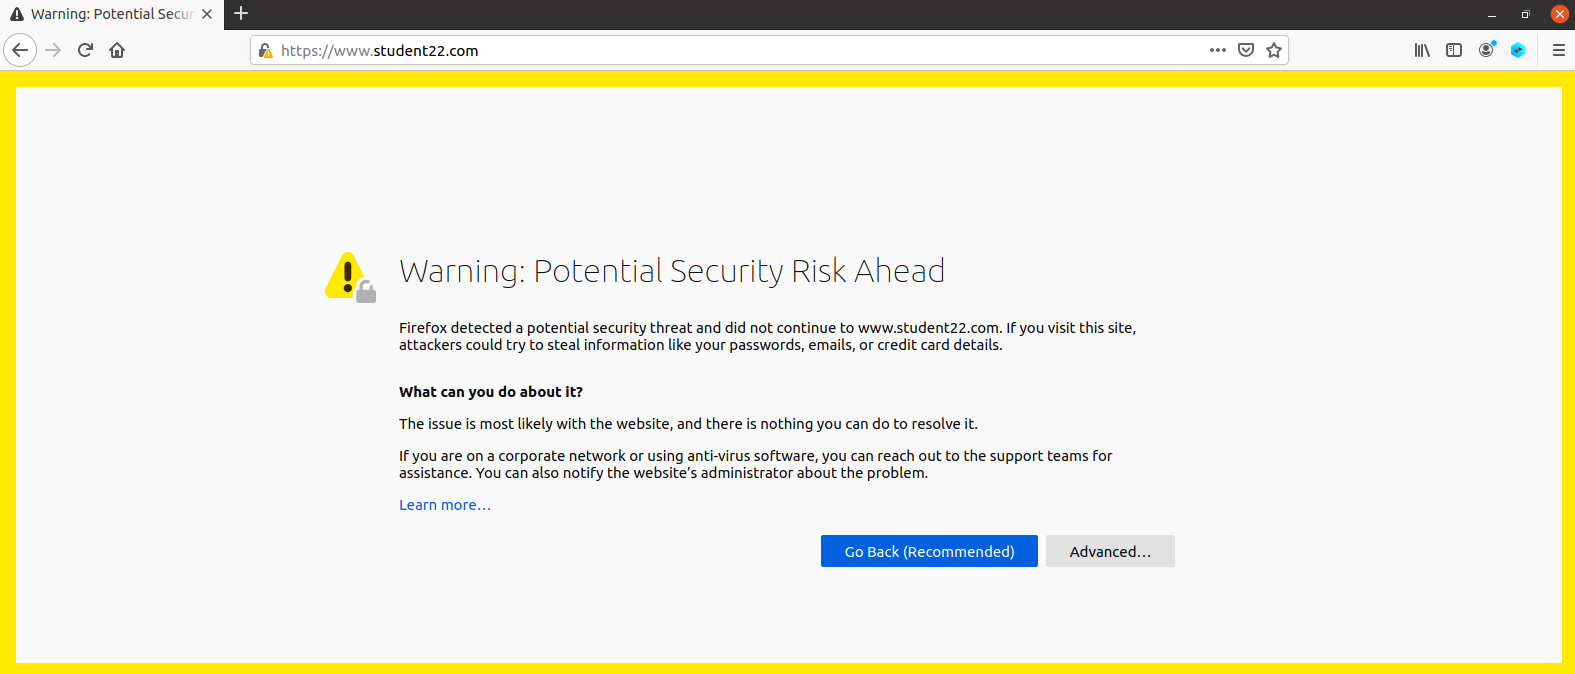
\includegraphics[height=\textheight,width=\textwidth,keepaspectratio]
    {figures/https_do_not_work.png}
    \caption{Cannot browse the HTTPS website at the first time.}
    \label{fig:https_do_not_work}
\end{figure}

\begin{figure}
    \centering
    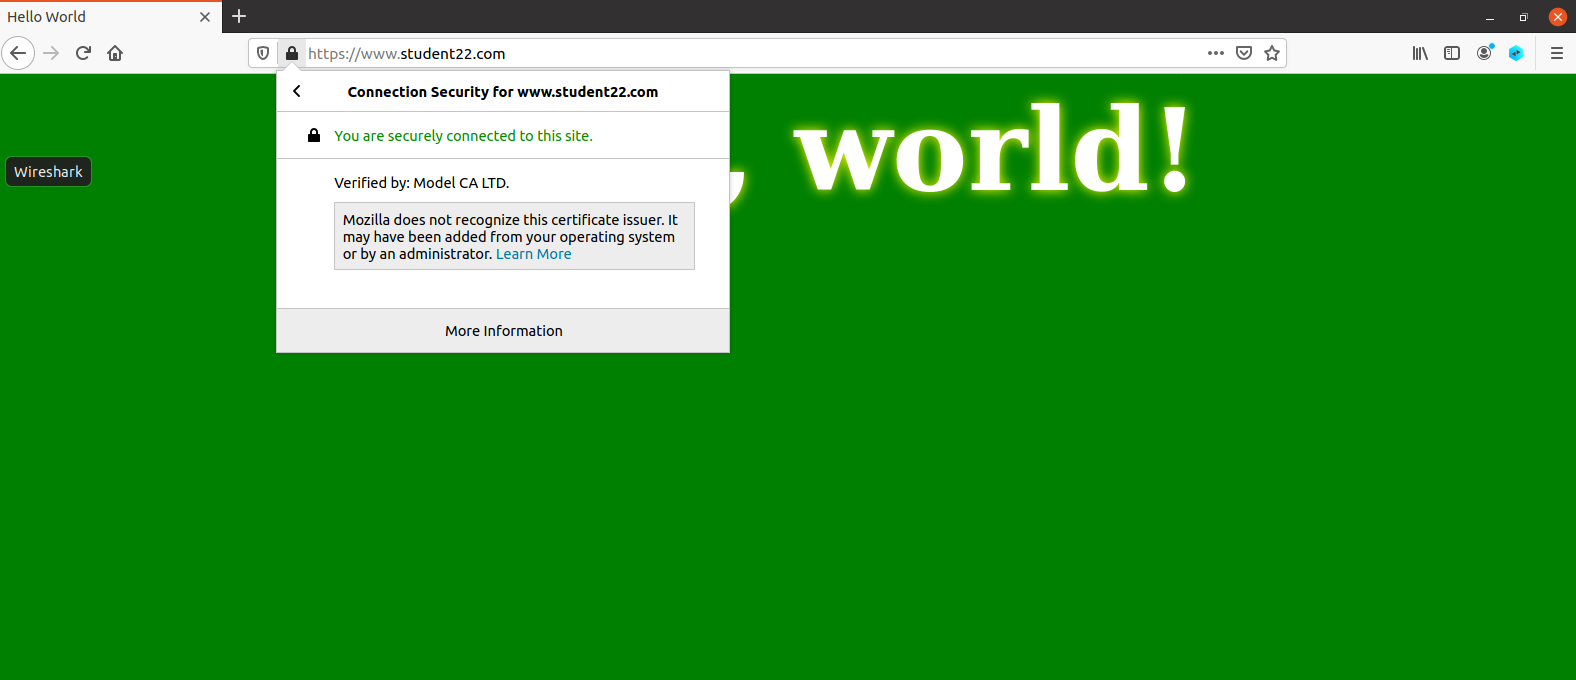
\includegraphics[height=\textheight,width=\textwidth,keepaspectratio]
    {figures/https_work.png}
    \caption{HTTPS website can be accessed after adding CA certificate to Firefox.}
    \label{fig:https_work}
\end{figure}

\begin{figure}
    \centering
    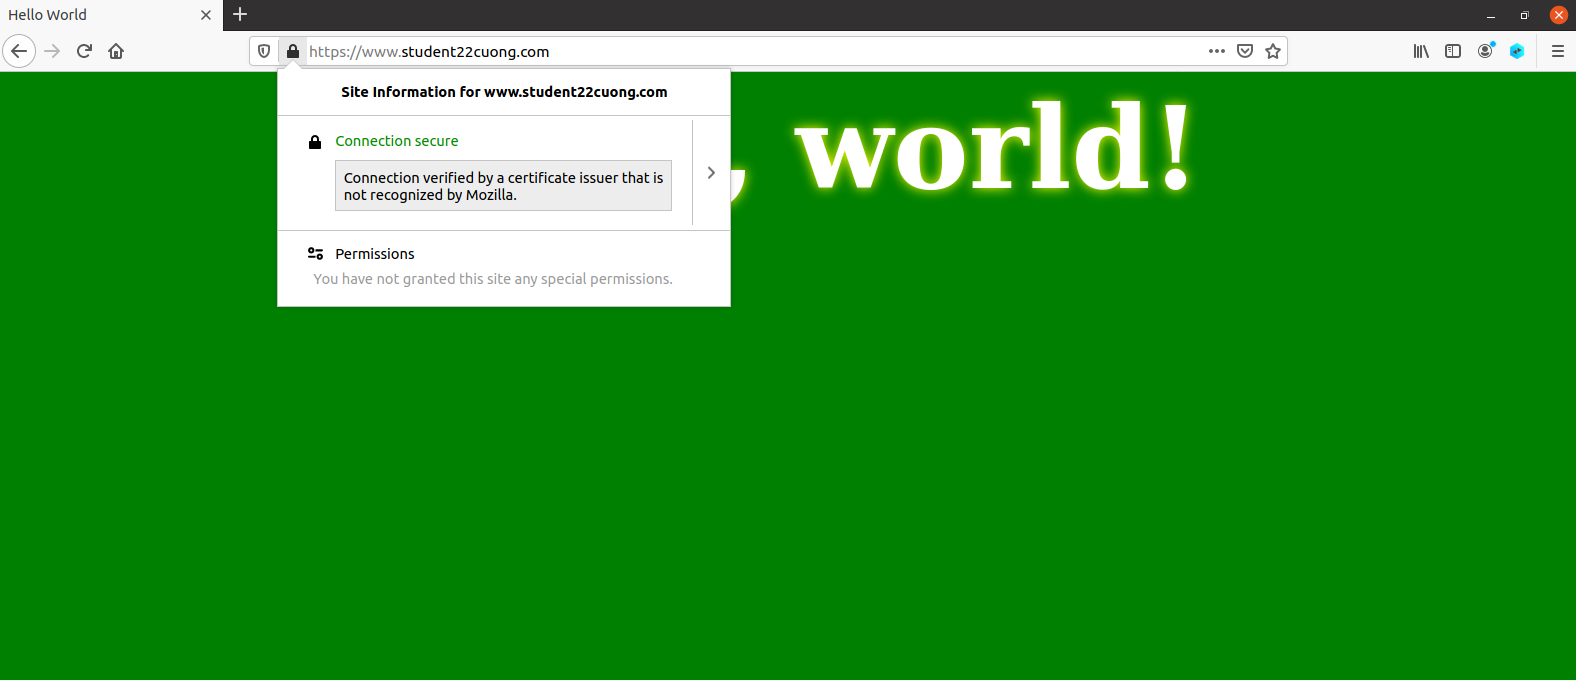
\includegraphics[height=\textheight,width=\textwidth,keepaspectratio]
    {figures/https_work_cuong.png}
    \caption{The first server alias can be accessed.}
    \label{fig:https_work_cuong}
\end{figure}

\begin{figure}
    \centering
    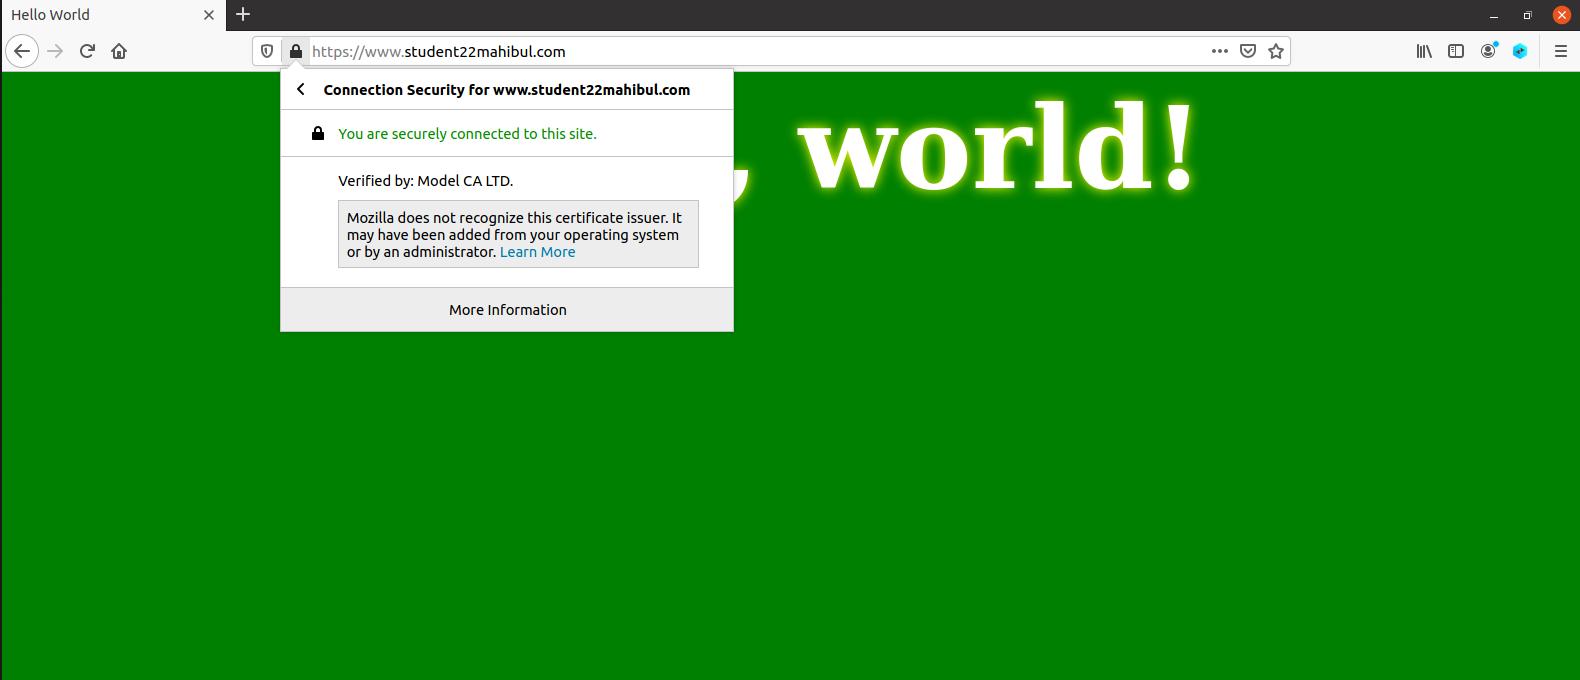
\includegraphics[height=\textheight,width=\textwidth,keepaspectratio]
    {figures/https_work_mahibul.png}
    \caption{The second server alias can be accessed.}
    \label{fig:https_work_mahibul}
\end{figure}

\begin{lstlisting}[caption=Append two alternative names to a list of known hosts.,
    label={lst:add_alt_name}]
    10.9.0.80 www.student22cuong.com
    10.9.0.80 www.student22mahibul.com
\end{lstlisting}

According to SEED's instruction, we modified the {\fontfamily{qcr}\selectfont
bank32\_apache\_ssl.conf} file (see \autoref{lst:server_config}).However, we
cannot access the HTTPS website {\fontfamily{qcr}\selectfont
www.student22.com} since the certificate of this website are not issued by
any of available CAs in Firefox (the browser we used in this case) and in Ubuntu OS.
To solve this problem, we included the root CA certificate which is created and
self-signed in previous Task 1 into Firefox. As a result, Firefox now can ask
our CA to verify the certificate of {\fontfamily{qcr}\selectfont
www.student22.com} (note that our CA signed this certificate in Task 3). Hence,
we can now access HTTPS website of {\fontfamily{qcr}\selectfont
www.student22.com} (see \autoref{fig:https_work}). In addition, after adding two
server aliases {\fontfamily{qcr}\selectfont www.student22cuong.com} and
{\fontfamily{qcr}\selectfont www.student22mahibul.com} in the list of known hosts
by modifying the {\fontfamily{qcr}\selectfont /etc/hosts} file (see \autoref{lst:add_alt_name})
, we now can visit the two corresponding alias servers as well (see
\autoref{fig:https_work_cuong} and \autoref{fig:https_work_mahibul}).